\documentclass[conference]{IEEEtran}
\IEEEoverridecommandlockouts
% The preceding line is only needed to identify funding in the first footnote. If that is unneeded, please comment it out.
\usepackage{cite}
\usepackage{amsmath,amssymb,amsfonts}
\usepackage{algorithmic}
\usepackage{graphicx}
\usepackage{textcomp}
\usepackage{xcolor}
\def\BibTeX{{\rm B\kern-.05em{\sc i\kern-.025em b}\kern-.08em
    T\kern-.1667em\lower.7ex\hbox{E}\kern-.125emX}}
\begin{document}

\title{Forecasting Total Energy Consumption in the Swiss Energy Grid}

\author{
\IEEEauthorblockN{Matthias Minder}
\IEEEauthorblockA{matthias.minder@epfl.ch}
\and
\IEEEauthorblockN{Yves Rychener}
\IEEEauthorblockA{
yves.rychener@epfl.ch}}


\maketitle

\begin{abstract}
TODO
\end{abstract}


\section{Introduction}
The energy grid is a highly complex network that has to be tightly controlled by the so-called grid operator in order to assure its well-functioning. In particular, energy consumption has to be at equilibrium with production at all times to avoid blackouts with possibly fatal consequences. It is therefore of great interest to accurately model and forecast the energy consumption, such that the energy made available to the grid can be adjusted accordingly. Moreover, long-term forecasting is of interest to adjust the energy strategy: How much power plants will be needed in the future and should be built? 
\par
Within the scope of this work, we therefore aim to generate accurate short- and long-term forecasts for the total energy consumption of the Swiss energy grid. To this effect, we analyze the quarter-hourly grid data between 2009 and 2019 available from the Swiss grid operator, Swissgrid [CITATION!]. The work will be structured as follows: In the second chapter, we present exploratory analysis of the data to identify sensible models. In the third chapter, we then [ DO WHAT?!?]. 

\section{Data Exploration}
\begin{figure*}[ht]
	\centering
	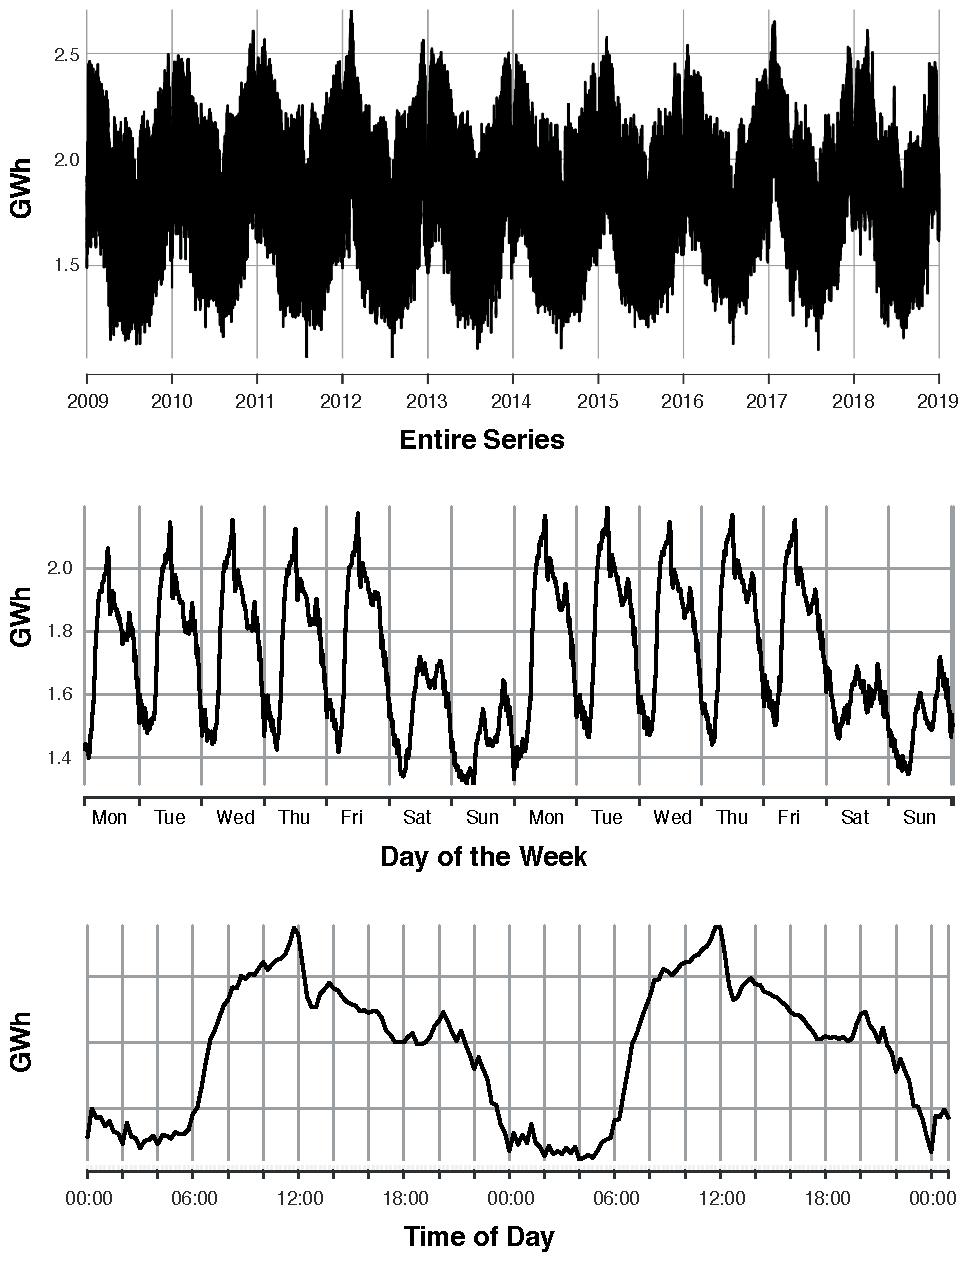
\includegraphics[width=0.8\textwidth]{Figs/Fig1.pdf}
	\caption{Total consumption in the Swiss Energy Grid, showing the entire series, two example weeks and two example work days.}
	\label{SeriesPlot}
\end{figure*}
The full time series for energy consumption together with representative weeks and days are shown in \ref{SeriesPlot}. From the plots, it becomes apparent that there are multiple levels of seasonality present in the data. First of all, we see a roughly sinusoidal yearly variation, with higher values during winter months than summer. Secondly, we see a weekly repetitive pattern, with lower energy consumption during the week-end as compared to the work days. Finally, we see a highly irregular daily pattern with the highest energy consumption right before lunchtime.
\par
Moreover, on the plot of the full time series we observe a sharp drop in energy consumption around Christmas and New Year. The same applies for other public holidays such as the first of August or  easter. Note that the public holidays vary from canton to canton, making it hard to identify them and model them separately. 
\par
A good model for short term predictions has to account for all of the aforementioned seasonal patterns and particularities and will therefore be challenging to construct. Within the scope of this report, we will try different approaches for modeling the seasonalities and the remaining residuals. 
\par



\begin{thebibliography}{00}

\item
\end{thebibliography}

\end{document}
